% =====================================================================
%  Data Mining · SGH · SMMD-ADA / SMMD-AAB   —   Block 5 slide deck
%  Template: Frankfurt + seahorse + miniframes (same as course template)
%
%  Compilation:
%    pdflatex block5.tex   (run twice for the section headline)
%
%  Figures: regenerate with   uv run python lecture_5/make_figures.py
%
%  Speaker-notes display modes (uncomment one):
%    \setbeameroption{hide notes}                          % slides only
%    \setbeameroption{show notes}                          % slides + note pages
%    \setbeameroption{show notes on second screen=right}   % presenter mode
%    \setbeameroption{show only notes}                     % notes printout
% =====================================================================
\documentclass[10pt,aspectratio=169]{beamer}

\usepackage[utf8]{inputenc}
\usepackage[T1]{fontenc}
\usepackage{booktabs}
\usepackage{array}
\usepackage{multirow}
\usepackage{amsmath,amssymb}
\usepackage{graphicx}
\usepackage{xcolor}
\usepackage{tikz}
\usetikzlibrary{arrows.meta,positioning,shapes.geometric}

% - Theme -
\usetheme{Frankfurt}
\usecolortheme{seahorse}
\useoutertheme{miniframes}
\setbeamertemplate{navigation symbols}{}
\setbeamertemplate{footline}[frame number]

% - Speaker notes -
\setbeameroption{hide notes}
% \setbeameroption{show notes on second screen=right}

% - Colours for figures -
\definecolor{sghblue}{RGB}{0,51,102}

% - Metadata -
\title[Data Mining]{Data Mining}
\subtitle{Block 5 - Pattern discovery \& text mining}
\author{Daniel Wlazło}
\institute{SGH Warsaw School of Economics - SMMD-ADA / SMMD-AAB}
\date{03 November 2026}

\begin{document}

% ============================================================
\begin{frame}[plain]
  \begin{center}
    \vspace{1cm}
    {\LARGE\textbf{Data Mining}}\\[0.5cm]
    {\large Block 5 - Pattern discovery \& text mining}\\[1.5cm]
    {\large Daniel Wlazło} \\[0.2cm]
    {\small SGH Warsaw School of Economics - SMMD-ADA / SMMD-AAB} \\[0.2cm]
    {\small 03 November 2026}
  \end{center}
\end{frame}

% ============================================================
\begin{frame}{Today, hour by hour}
  \begin{enumerate}
    \item \textbf{Recap} - the unsupervised rules of engagement \hfill {\small$\sim$5 min}
    \item \textbf{Baskets} - which products travel together \hfill {\small$\sim$25 min}
    \item \textbf{Rules \& their three numbers} - support, confidence, lift \hfill {\small$\sim$30 min}
    \item \textbf{Mining at scale} - Apriori \& FP-Growth \hfill {\small$\sim$15 min}
    \item \textbf{Text becomes numbers} - tokens, bags, TF-IDF \hfill {\small$\sim$35 min}
    \item \textbf{Classifying complaints} - multiclass, delivered \hfill {\small$\sim$20 min}
    \item \textbf{Pitfalls} - rules on noise, text hygiene \hfill {\small$\sim$15 min}
    \item \textbf{Lab} - notebook \texttt{05\_pattern\_mining\_text} \hfill {\small$\sim$35 min}
  \end{enumerate}
  \vspace{0.3em}
  \begin{center}\small Breaks roughly every 50 minutes.\end{center}
\end{frame}

% ============================================================
\begin{frame}{Last week in five sentences}
  \begin{enumerate}
    \item Without labels there is no ``correct'' - only \textbf{useful},
          argued via internal metrics, stability, and business sense.
    \item \textbf{Distance is a modelling choice}; unscaled features make
          it for you.
    \item K-means \textbf{always answers}; silhouette and stability tell you
          how much to believe it.
    \item Assumptions decide what each tool can see - and \textbf{PCA}
          can only compress redundancy.
    \item Always ask: \emph{what would this deliverable look like on
          noise?}
  \end{enumerate}
  \vspace{0.5em}
  \begin{center}
    Today: two new kinds of structure - \alert{co-occurrence} and
    \alert{text} - and a supervised comeback you were promised in Block 1.
  \end{center}
\end{frame}

% ============================================================
% SECTION: BASKETS
% ============================================================
\section{Baskets}

% ---------------------------------------------------------------
\begin{frame}{The cross-selling question}
  \begin{itemize}
    \item New data, same 4{,}000 customers: which of ten \alert{products}
          each of them holds - checking, savings, cards, loans, mortgage,
          insurance, brokerage, deposits.
    \item The business question: \emph{which products travel together} -
          and which pairing is a genuine opportunity rather than a
          coincidence of popularity?
    \item Uses: cross-sell campaigns, bundling, product-page ``customers
          also hold'', early-warning (a product mix that predicts churn).
    \item Loaded via \texttt{finance\_data.load\_baskets()} - one row per
          customer, one 0/1 column per product.
  \end{itemize}
\end{frame}

% ---------------------------------------------------------------
\begin{frame}{Where else baskets appear}
  \begin{itemize}
    \item \textbf{Retail} - the literal shopping basket; the field's
          birthplace and name.
    \item \textbf{Pharmacy \& medicine} - co-prescribed drugs,
          co-occurring diagnoses.
    \item \textbf{Web \& apps} - pages visited in one session; features
          used by one account.
    \item \textbf{Fraud} - devices, addresses and phone numbers shared
          across applications: co-occurrence as a \alert{ring detector}.
  \end{itemize}
  \vspace{0.5em}
  \begin{center}
    The abstraction is one table: \alert{transactions $\times$ items},
    binary. Whoever can build that table can mine it.
  \end{center}
\end{frame}

% ---------------------------------------------------------------
\begin{frame}[fragile]{Building the matrix}
  \small Ours arrives ready (one row per customer, 0/1 per product). In the
  wild, baskets arrive as \emph{lists} - then:
{\footnotesize
\begin{semiverbatim}
from mlxtend.preprocessing import TransactionEncoder

te = TransactionEncoder()
X = te.fit(transactions).transform(transactions)   \textit{\# lists -> 0/1 matrix}
baskets = pd.DataFrame(X, columns=te.columns_)
\end{semiverbatim}}
  \vspace{0.3em}
  \begin{itemize}\small
    \item Long transactional tables (customer, product, date) become
          baskets with one \texttt{pd.crosstab} - but first answer
          Block 1's question: \alert{what is a row?} One visit? One
          customer-lifetime? The rules you find inherit the answer.
  \end{itemize}
\end{frame}

% ---------------------------------------------------------------
\begin{frame}{The basket matrix}
  \begin{center}
    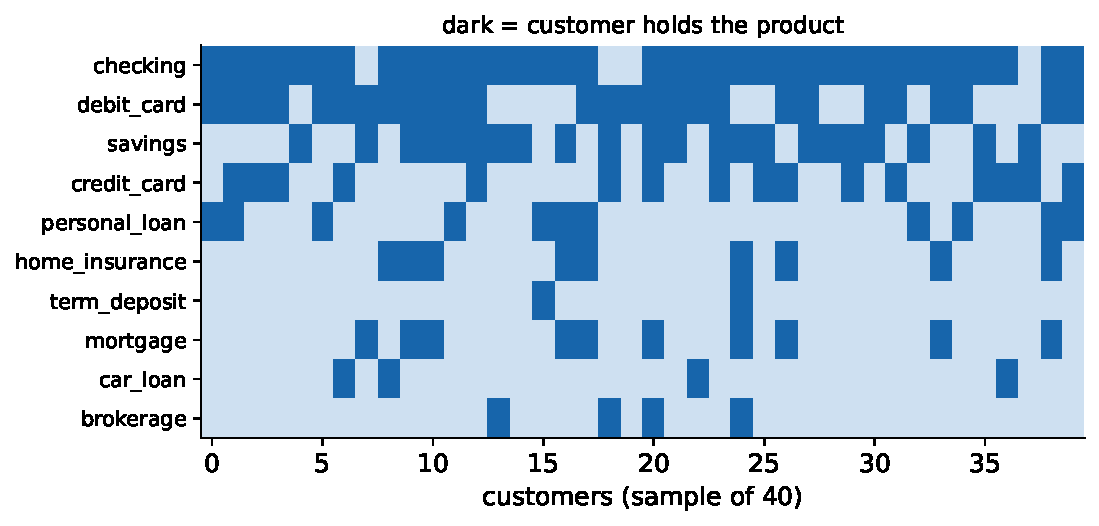
\includegraphics[width=0.78\textwidth]{figures/fig_basket_sample.pdf}
  \end{center}
  \begin{itemize}\small
    \item Binary and \alert{sparse} - most customers hold few products.
          (Retail is sparser still: thousands of items, baskets of five.)
    \item Every technique today starts from exactly this matrix.
  \end{itemize}
\end{frame}

% ---------------------------------------------------------------
\begin{frame}{Support: how common is a combination?}
  \begin{center}
    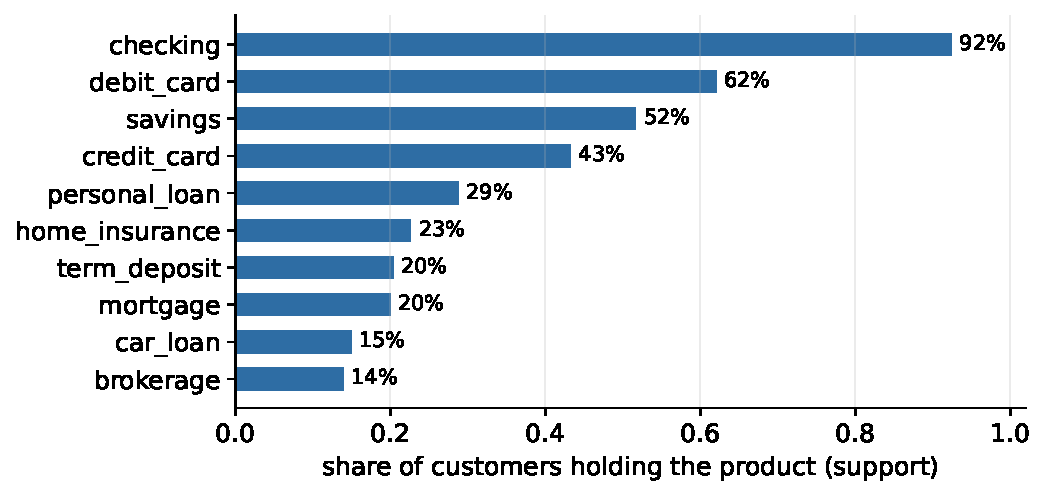
\includegraphics[width=0.7\textwidth]{figures/fig_penetration.pdf}
  \end{center}
  \begin{itemize}\small
    \item An \textbf{itemset} is any set of products; its \textbf{support}
          = share of customers holding all of it:
          $\text{supp}(A) = n_A / n$.
    \item Single-item supports are just penetration rates. The interesting
          ones are combinations: $\text{supp}(\{\text{mortgage,
          insurance}\}) = 17\%$.
  \end{itemize}
\end{frame}

% ---------------------------------------------------------------
\begin{frame}{From itemsets to rules}
  \begin{itemize}
    \item A \textbf{rule} $A \Rightarrow B$: customers holding $A$ tend to
          also hold $B$. ($A$: antecedent, $B$: consequent.)
    \item The arrow is \alert{our reading direction, not causality} -
          the data only says the products co-occur; the sale process, not
          the mortgage, causes the insurance.
    \item Every itemset spawns many rules
          ($\{a,b,c\}$: $a\Rightarrow bc$, $ab \Rightarrow c$, \ldots) -
          we need numbers to rank them.
  \end{itemize}
  \vspace{0.6em}
  \begin{center}
    Three numbers, next slide - the exam will ask for all three.
  \end{center}
\end{frame}

% ---------------------------------------------------------------
\begin{frame}{Sequences: baskets with a clock (mention)}
  \begin{itemize}
    \item Our matrix is a snapshot - \emph{what is held now}. Add
          timestamps and the question upgrades: \alert{what comes next?}
          (checking $\to$ debit card $\to$ first savings $\to$ mortgage).
    \item Sequence mining (PrefixSpan and friends) finds ordered patterns;
          next-best-product models are its supervised cousins.
    \item Why banks care: the \emph{order} is the customer lifecycle -
          and interventions live between the steps.
    \item Today we stay with snapshots; know that the clocked version
          exists.
  \end{itemize}
\end{frame}

% ============================================================
% SECTION: RULES
% ============================================================
\section{Rules}

% ---------------------------------------------------------------
\begin{frame}{The three numbers of a rule $A \Rightarrow B$}
  \[
    \text{support} = \frac{n_{A \cup B}}{n}
    \qquad
    \text{confidence} = \frac{n_{A \cup B}}{n_A} = P(B \mid A)
    \qquad
    \text{lift} = \frac{P(B \mid A)}{P(B)}
  \]
  \vspace{0.3em}
  \begin{itemize}
    \item \textbf{Support} - how much of the portfolio the rule touches:
          \alert{materiality}.
    \item \textbf{Confidence} - how reliably $A$-holders hold $B$:
          \alert{precision of the promise}.
    \item \textbf{Lift} - how much more often than \emph{chance}:
          \alert{is there any relationship at all?}
          Lift $= 1$: independence; $> 1$: attraction; $< 1$: repulsion.
  \end{itemize}
  \vspace{0.4em}
  \begin{center}\small
    Mnemonic: support = size, confidence = reliability, lift = surprise.
  \end{center}
\end{frame}

% ---------------------------------------------------------------
\begin{frame}{Worked example, by hand (ours)}
  Out of $n = 4{,}000$ customers: $n_{\text{mortgage}} = 800$,
  $n_{\text{insurance}} = 906$, both $= 678$.
  \[
    \text{supp} = \frac{678}{4000} = 0.17
    \qquad
    \text{conf} = \frac{678}{800} = 0.85
    \qquad
    \text{lift} = \frac{0.85}{906/4000} = \frac{0.85}{0.227} \approx 3.7
  \]
  \begin{itemize}\small
    \item Read it aloud: \emph{17\% of customers hold both; 85\% of
          mortgage holders have the insurance - 3.7$\times$ more often
          than a random customer.}
    \item Business translation: the bundle works at the mortgage desk.
          The actionable rule is its \alert{absence}: chase the 15\% of
          mortgage holders \emph{without} insurance.
  \end{itemize}
\end{frame}

% ---------------------------------------------------------------
\begin{frame}{Your turn: brokerage $\Rightarrow$ term deposit}
  Out of $n = 4{,}000$: $n_{\text{brokerage}} = 558$,
  $n_{\text{deposit}} = 815$, both $= 359$.
  \vspace{0.4em}
  \begin{center}
    \emph{Compute support, confidence, lift. Sixty seconds.}
  \end{center}
  \vspace{0.4em}
  \pause
  \[
    \text{supp} = \frac{359}{4000} \approx 0.09
    \qquad
    \text{conf} = \frac{359}{558} \approx 0.64
    \qquad
    \text{lift} = \frac{0.64}{815/4000} \approx 3.2
  \]
  \begin{itemize}\small
    \item Weaker promise than the mortgage rule (64\% vs 85\%) but the same
          verdict: a real affinity - the \alert{affluent-saver} pattern,
          which Block 4's segmentation already sketched.
  \end{itemize}
\end{frame}

% ---------------------------------------------------------------
\begin{frame}{The confidence trap}
  A rule from our data:
  \begin{center}
    \texttt{savings} $\Rightarrow$ \texttt{checking}
    \qquad confidence $= \alert{92.7\%}$
  \end{center}
  \vspace{0.3em}
  \begin{itemize}
    \item Sounds spectacular - until you notice \alert{92.4\% of
          everyone} has a checking account. Lift $= 1.003$: pure
          independence.
    \item High confidence toward a \emph{popular} consequent is base-rate
          flattery - Block 2's accuracy trap wearing a basket.
    \item Rule hygiene: \textbf{filter by support} (materiality),
          \textbf{rank by lift} (surprise), \textbf{read confidence} for
          the campaign promise.
  \end{itemize}
\end{frame}

% ---------------------------------------------------------------
\begin{frame}{The rule landscape}
  \begin{center}
    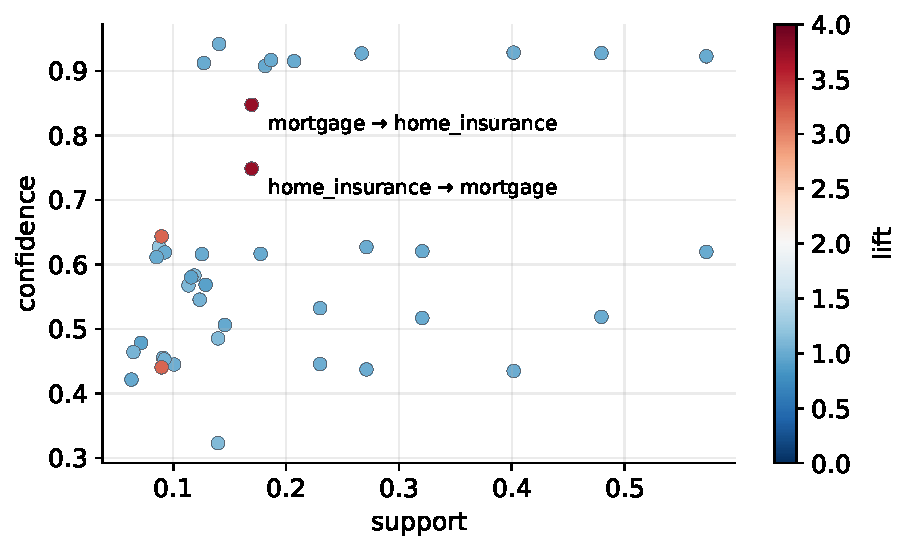
\includegraphics[width=0.56\textwidth]{figures/fig_rules_scatter.pdf}
  \end{center}
  \begin{itemize}\small
    \item Every dot is a single-item rule; the two red-hot dots are the
          mortgage--insurance pair, in both reading directions.
    \item The crowd at lift $\approx 1$ is what most rules look like:
          popular items co-occurring by \alert{arithmetic}, not affinity.
  \end{itemize}
\end{frame}

% ---------------------------------------------------------------
\begin{frame}{Top rules by lift - and how to read a rule list}
  \begin{center}
    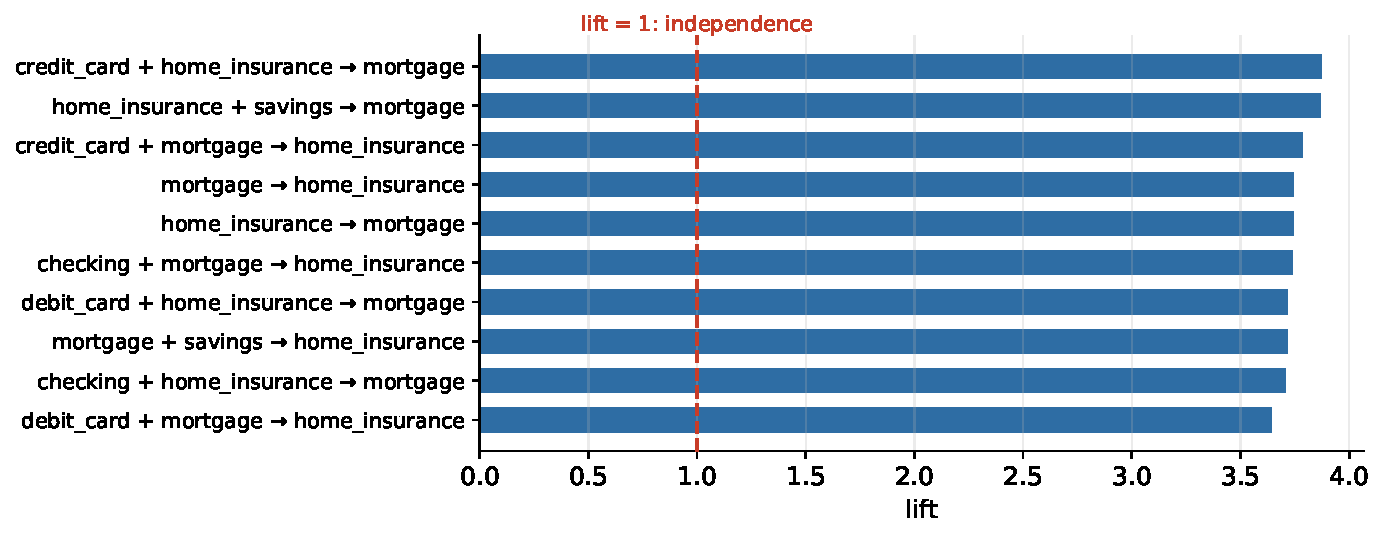
\includegraphics[width=0.82\textwidth]{figures/fig_top_rules.pdf}
  \end{center}
  \begin{itemize}\small
    \item Notice the \alert{redundancy}: the same mortgage--insurance
          affinity appears in both directions and re-decorated with
          irrelevant extras (\texttt{+ checking}, \texttt{+ debit\_card}).
    \item One relationship, many rules - deduplicate before reporting,
          or the deck of ``insights'' is one insight in ten costumes.
  \end{itemize}
\end{frame}

% ---------------------------------------------------------------
\begin{frame}{Beyond the big three (mentions)}
  \begin{itemize}
    \item \textbf{Leverage}: $P(A \cap B) - P(A)P(B)$ - lift's additive
          sibling; harder to fool with tiny supports.
    \item \textbf{Conviction}:
          $\dfrac{1 - \text{supp}(B)}{1 - \text{conf}(A \Rightarrow B)}$
          - how much more often the rule would be wrong under
          independence ($=1$: independent; $\to\infty$: never wrong).
    \item \textbf{Closed / maximal itemsets}: compressed inventories of
          frequent sets - the cure for rule explosion.
    \item With $p$ products there are $2^p - 1$ itemsets; at $p = 10$
          that's 1{,}023, at retail scale it's astronomy -
          \alert{multiple testing is built into the method}. (The sobering
          demo waits in the pitfalls section.)
  \end{itemize}
\end{frame}

% ---------------------------------------------------------------
\begin{frame}{From rule to campaign - honestly}
  \begin{itemize}
    \item The action hides in the rule's \alert{complement}: 15\% of
          mortgage holders lack the insurance - that is the call list.
    \item But the rule is co-occurrence, not causality: those 15\% may
          differ \emph{exactly} in whatever made them decline the bundle.
    \item The honest upgrade: run the campaign as an \alert{experiment} -
          hold out a random control group, measure uplift, not response.
    \item And expect \alert{feedback}: acting on a pattern changes it
          (every mined rule fades as campaigns exploit it) -
          re-mine on fresh data, date every rule list.
  \end{itemize}
  \vspace{0.4em}
  \begin{center}\small
    Association rules \emph{nominate} actions; experiments
    \emph{validate} them.
  \end{center}
\end{frame}

% ============================================================
% SECTION: MINING
% ============================================================
\section{Mining}

% ---------------------------------------------------------------
\begin{frame}{Why brute force dies}
  \begin{itemize}
    \item Counting support for every one of the $2^p - 1$ itemsets - at
          a supermarket's $p = 30{,}000$ - means the universe ends
          first.
    \item Yet stores mine baskets every night. The rescue is one
          observation about support:
  \end{itemize}
  \vspace{0.6em}
  \begin{block}{The Apriori principle (downward closure)}
    Every subset of a frequent itemset is frequent. Equivalently: if an
    itemset is infrequent, \alert{every superset is infrequent too} -
    and can be skipped without counting.
  \end{block}
  \vspace{0.4em}
  \begin{center}\small
    If \{brokerage, car\_loan\} is rare, \{brokerage, car\_loan,
    \emph{anything}\} is rare. No need to look.
  \end{center}
\end{frame}

% ---------------------------------------------------------------
\begin{frame}{Apriori by hand: one level (exam-friendly)}
  Five customers, min\_support $= 40\%$ (i.e.\ $\geq 2$ of 5):
  \begin{center}\small
  \begin{tabular}{@{}lc|lc@{}}
    \toprule
    1-itemset & supp & candidate 2-itemset & supp \\
    \midrule
    \{card\} & 4/5 \checkmark & \{card, loan\} & 3/5 \checkmark \\
    \{loan\} & 3/5 \checkmark & \{card, deposit\} & 2/5 \checkmark \\
    \{deposit\} & 2/5 \checkmark & \{loan, deposit\} & 1/5 \texttimes \\
    \{leasing\} & 1/5 \texttimes & \multicolumn{2}{l}{\{leasing, \emph{anything}\}: \alert{never generated}} \\
    \bottomrule
  \end{tabular}
  \end{center}
  \vspace{0.4em}
  \begin{itemize}\small
    \item Level 3: only \{card, loan, deposit\} is even a candidate -
          and it dies because its subset \{loan, deposit\} already failed.
    \item That is the whole algorithm: count a level, prune, build the
          next level \alert{only from survivors}.
  \end{itemize}
\end{frame}

% ---------------------------------------------------------------
\begin{frame}{Apriori and FP-Growth}
  \begin{columns}[T]
    \begin{column}{0.5\textwidth}
      \textbf{Apriori (1994)}
      \begin{itemize}\small
        \item level-wise: frequent 1-itemsets $\to$ candidate 2-itemsets
              $\to$ \ldots
        \item prunes with downward closure at every level
        \item repeatedly re-scans the data - simple, parallel-friendly,
              I/O heavy
      \end{itemize}
    \end{column}
    \begin{column}{0.5\textwidth}
      \textbf{FP-Growth (2000)}
      \begin{itemize}\small
        \item compresses baskets into a \alert{prefix tree} (FP-tree)
        \item mines the tree recursively - no candidate generation
        \item two data scans total; the usual industrial choice
      \end{itemize}
    \end{column}
  \end{columns}
  \vspace{0.7em}
  \begin{center}
    Same definition, same output - only the route differs.
    \texttt{mlxtend} ships both; at our $p = 10$, either is instant.
  \end{center}
\end{frame}

% ---------------------------------------------------------------
\begin{frame}{Practical mining decisions}
  \begin{itemize}
    \item \textbf{\texttt{min\_support} is a business number}: ``rules
          touching $<$3\% of customers can't fund a campaign'' - set it
          from materiality, not from what makes the list look rich.
    \item Too low: rule explosion and noise. Too high: only the obvious
          survives (\texttt{checking} co-occurs with everything).
    \item \textbf{Long-tail reality}: in retail, most interesting items
          are individually rare - category-level mining (``any insurance
          product'') is the standard fix.
    \item \textbf{Output discipline}: filter support $\to$ rank lift
          $\to$ deduplicate mirrors and supersets $\to$ \emph{then} read.
  \end{itemize}
\end{frame}

% ============================================================
% SECTION: TEXT
% ============================================================
\section{Text}

% ---------------------------------------------------------------
\begin{frame}{The other unstructured eighty percent}
  \begin{itemize}
    \item Banks are full of text nobody mines: complaints, chat
          transcripts, advisor notes, application free-text fields.
    \item Our new corpus: \alert{1{,}200 customer complaints}, each labelled
          with one of five categories - card fraud, mortgage, fees, app
          \& service, collections
          (\texttt{finance\_data.load\_complaints()}).
    \item Business task waiting at the end: \alert{route each complaint to
          the right team} - the multiclass classification promised on
          Block 1's map.
    \item But models eat numbers. The whole craft of text mining is the
          bridge: \alert{strings $\to$ a feature matrix}.
  \end{itemize}
\end{frame}

% ---------------------------------------------------------------
\begin{frame}{The bridge, in four steps}
  \begin{enumerate}
    \item \textbf{Normalise} - lowercase, strip punctuation; decisions,
          not defaults (is ``PLN'' a word? is ``24/7''?).
    \item \textbf{Tokenise} - split into words (or word pieces; or
          characters).
    \item \textbf{Count} - one column per token, one row per document:
          the \alert{bag of words}.
    \item \textbf{Weigh} - damp the ubiquitous, boost the distinctive:
          \alert{TF-IDF}.
  \end{enumerate}
  \vspace{0.5em}
  \begin{center}
    Each step throws information away \emph{on purpose} - the art is
    knowing what you can afford to lose. (Step 3 loses word order;
    n-grams buy some of it back.)
  \end{center}
\end{frame}

% ---------------------------------------------------------------
\begin{frame}{Normalisation decisions: stopwords, stems, lemmas}
  \begin{itemize}
    \item \textbf{Stopwords} - dropping \emph{the, my, and} shrinks the
          matrix; dropping \alert{not} reverses meanings
          (``\emph{not} refunded''). Audit any default list before
          trusting it.
    \item \textbf{Stemming} - chop endings by rule
          (\emph{charged, charges, charging} $\to$ \emph{charg});
          fast, crude, occasionally comic.
    \item \textbf{Lemmatisation} - dictionary-based reduction to base
          forms; slower, cleaner, and where morphology is rich
          (Polish: \emph{opłata, opłaty, opłatom, opłatach}) it earns its
          keep.
    \item Each choice merges columns of the future matrix - i.e.\ it is
          \alert{feature engineering}, with the same rule as always:
          document the recipe.
  \end{itemize}
\end{frame}

% ---------------------------------------------------------------
\begin{frame}{Bag of words}
  \begin{itemize}
    \item Document $\to$ vector of token counts; corpus $\to$ a
          \alert{documents $\times$ vocabulary} matrix - wide, sparse,
          non-negative. (Structurally: the basket matrix again! words are
          the items.)
    \item Lost on purpose: word order. ``the bank closed my account'' and
          ``my account closed the bank'' are the same bag.
    \item Kept: the lexical fingerprint - which turns out to carry most
          of the signal for routing-style tasks.
    \item sklearn: \texttt{CountVectorizer} - a transformer;
          \texttt{fit} learns the vocabulary, \texttt{transform} counts.
          (You already know this API.)
  \end{itemize}
\end{frame}

% ---------------------------------------------------------------
\begin{frame}{Zipf's law: every corpus looks like this}
  \begin{center}
    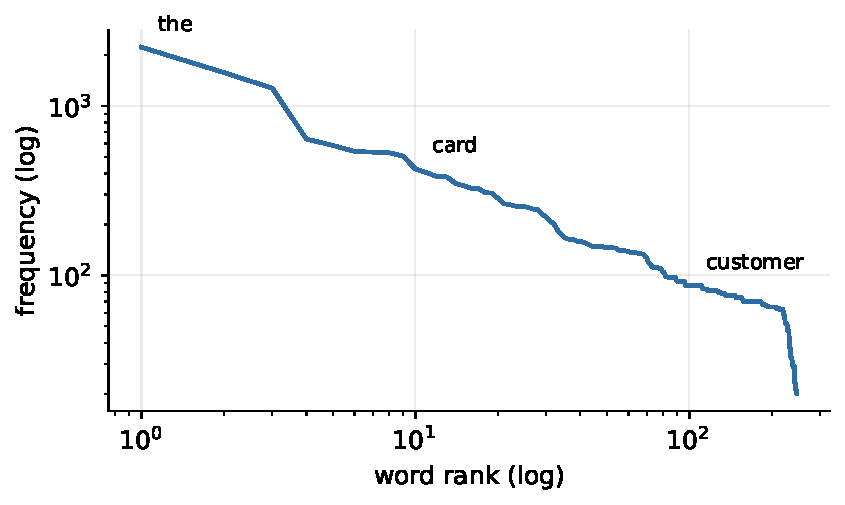
\includegraphics[width=0.58\textwidth]{figures/fig_zipf.pdf}
  \end{center}
  \begin{itemize}\small
    \item A few words are everywhere (\texttt{the}, \texttt{my},
          \texttt{account}); most words are rare. Log-log $\Rightarrow$
          near-straight line.
    \item Both ends are trouble: the head carries no distinction, the tail
          no statistics. \texttt{max\_df} and \texttt{min\_df} are the
          vectoriser's \alert{leash} - prune both ends.
  \end{itemize}
\end{frame}

% ---------------------------------------------------------------
\begin{frame}{TF-IDF: damp the common, boost the distinctive}
  \[
    w_{d,t} \;=\; \underbrace{\text{tf}_{d,t}}_{\text{count in doc}}
    \;\times\;
    \underbrace{\Bigl(\ln\frac{1 + n_{\text{docs}}}{1 + n_{\text{docs with } t}} + 1\Bigr)}_{\text{idf: rarity weight}}
  \]
  \begin{center}
    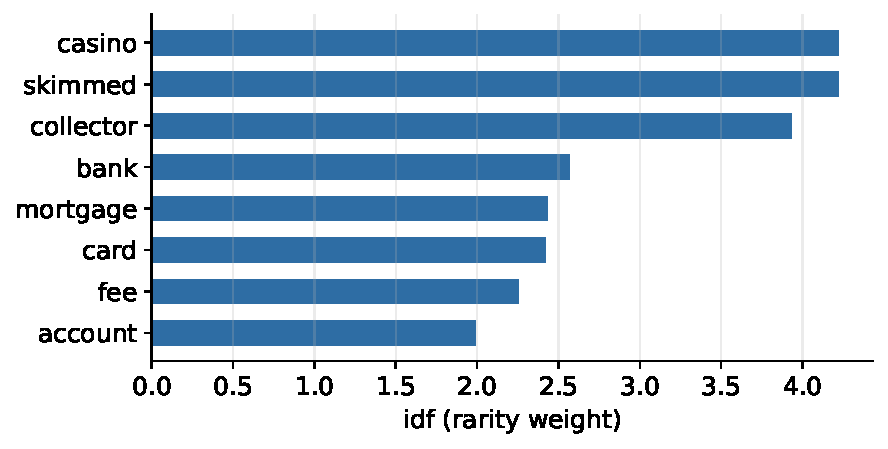
\includegraphics[width=0.48\textwidth]{figures/fig_idf_words.pdf}
  \end{center}
  \begin{itemize}\small
    \item In our corpus: \texttt{account} and \texttt{bank} cost almost
          nothing; \texttt{skimmed} and \texttt{casino} are expensive -
          and scream ``card fraud''.
    \item Plus length normalisation, so a rambling complaint doesn't
          outweigh a terse one.
  \end{itemize}
\end{frame}

% ---------------------------------------------------------------
\begin{frame}{N-grams: buying back word order}
  \begin{center}
    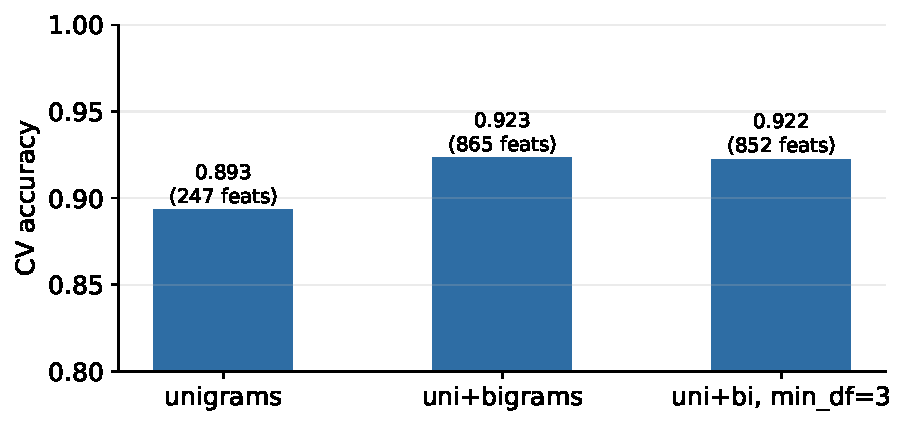
\includegraphics[width=0.66\textwidth]{figures/fig_ngram_effect.pdf}
  \end{center}
  \begin{itemize}\small
    \item Bigrams recover phrases the bag destroys -
          \emph{collection calls}, \emph{unauthorized transactions} -
          worth $+3$ points of accuracy here.
    \item The price: the vocabulary explodes ($247 \to 865$ features on
          1{,}200 documents). \texttt{min\_df} is the leash - our
          template corpus has a short tail ($865 \to 852$), but real
          corpora shed \emph{thousands} of one-off tokens with no accuracy
          loss.
  \end{itemize}
\end{frame}

% ---------------------------------------------------------------
\begin{frame}{Why $1{,}200 \times 865$ doesn't hurt: sparsity}
  \begin{itemize}
    \item A complaint uses $\sim$25 distinct words of the 247-word
          vocabulary (865 features with bigrams) - the matrix is
          \alert{$\sim$90--97\% zeros}.
    \item Sparse storage (CSR) keeps only the non-zeros: megabytes, not
          gigabytes; a retail-scale corpus (millions $\times$ 100k) still
          fits.
    \item Linear models multiply only the stored entries - which is
          \emph{why} logistic regression on text is fast, and one more
          reason linear wins wide-and-sparse country.
    \item Practical corollary: don't \texttt{.toarray()} a sparse matrix
          ``just to look'' - that is how notebooks die (Block 1's
          craft, text edition).
  \end{itemize}
\end{frame}

% ---------------------------------------------------------------
\begin{frame}{Distance between documents: cosine}
  \begin{itemize}
    \item Euclidean distance punishes \alert{length}: a long and a short
          complaint about the same fraud land far apart.
    \item Cosine similarity compares \alert{direction} - the mix of
          words, not the amount of them:
          $\cos(\theta) = \frac{x \cdot y}{\lVert x \rVert\, \lVert y \rVert}$.
    \item This is Block 4's ``distance is a modelling choice'', text
          edition - and the standard choice for TF-IDF vectors.
    \item Everything distance-based now applies to documents: cluster
          complaints (k-means on TF-IDF), find near-duplicates, build
          ``similar cases'' lookups.
  \end{itemize}
\end{frame}

% ---------------------------------------------------------------
\begin{frame}{Text is columns now - the whole course applies}
  Once text is a matrix, Blocks 1--4 come along for free:
  \small
  \begin{center}
  \begin{tabular}{@{}lll@{}}
    \toprule
    Technique & On text becomes & Block \\
    \midrule
    EDA & top words, Zipf, lengths per class & 1 \\
    Logistic regression & complaint routing (next section) & 2 \\
    Trees / GBDT & rarely better on sparse text - linear wins & 3 \\
    Clustering & topic-ish complaint groups & 4 \\
    PCA (as truncated SVD) & ``latent semantic'' axes - LSA & 4 \\
    \bottomrule
  \end{tabular}
  \end{center}
  \vspace{0.5em}
  \begin{center}
    One craft - representation - unlocks the entire toolbox.
  \end{center}
\end{frame}

% ============================================================
% SECTION: CLASSIFY
% ============================================================
\section{Classify}

% ---------------------------------------------------------------
\begin{frame}{Multiclass, delivered}
  \begin{itemize}
    \item Block 1 promised it, today pays: \texttt{category} $\in$
          \{card\_fraud, mortgage, fees, app\_service, collections\} -
          \alert{five classes}, one label each.
    \item The pipeline is two familiar pieces:
  \end{itemize}
  \vspace{0.3em}
  \begin{center}\small
    \texttt{make\_pipeline(TfidfVectorizer(), LogisticRegression())}
  \end{center}
  \vspace{0.3em}
  \begin{itemize}
    \item Logistic handles multiclass natively (one score per class,
          softmax picks); wide-and-sparse is \alert{linear-model country}
          - thousands of columns, each weakly informative, is exactly
          what regularised linear models digest best.
    \item Same golden rule, text edition: the vectoriser is \alert{fitted
          on training data only} - vocabulary leaks too.
  \end{itemize}
\end{frame}

% ---------------------------------------------------------------
\begin{frame}{Results: routing at 90\%}
  \begin{center}
    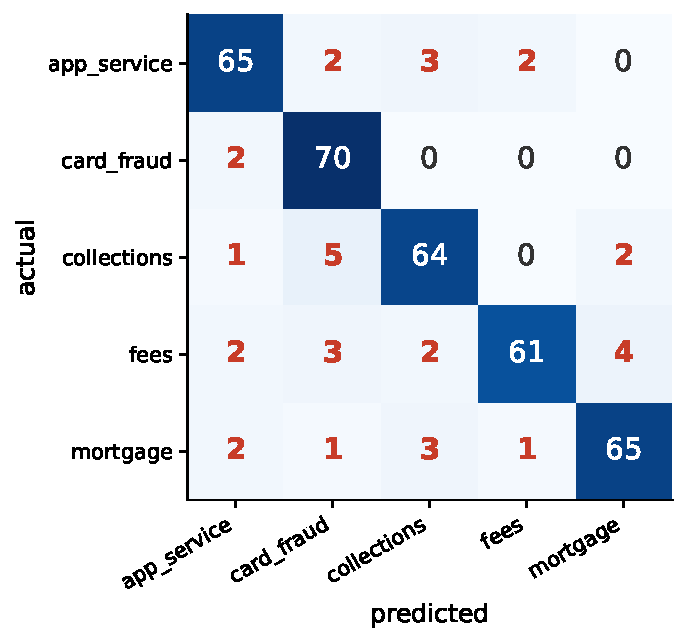
\includegraphics[width=0.36\textwidth]{figures/fig_confusion_text.pdf}
  \end{center}
  \begin{itemize}\small
    \item Test accuracy \alert{90\%} on five balanced classes (chance:
          20\%). Errors concentrate where complaints \emph{ramble} across
          topics - exactly the hard cases a human router also flags.
    \item Balanced classes make accuracy honest here; real complaint
          streams are imbalanced - then per-class recall and macro-F1
          take over (Block 2--3 reflexes).
  \end{itemize}
\end{frame}

% ---------------------------------------------------------------
\begin{frame}{What the model reads}
  \begin{center}
    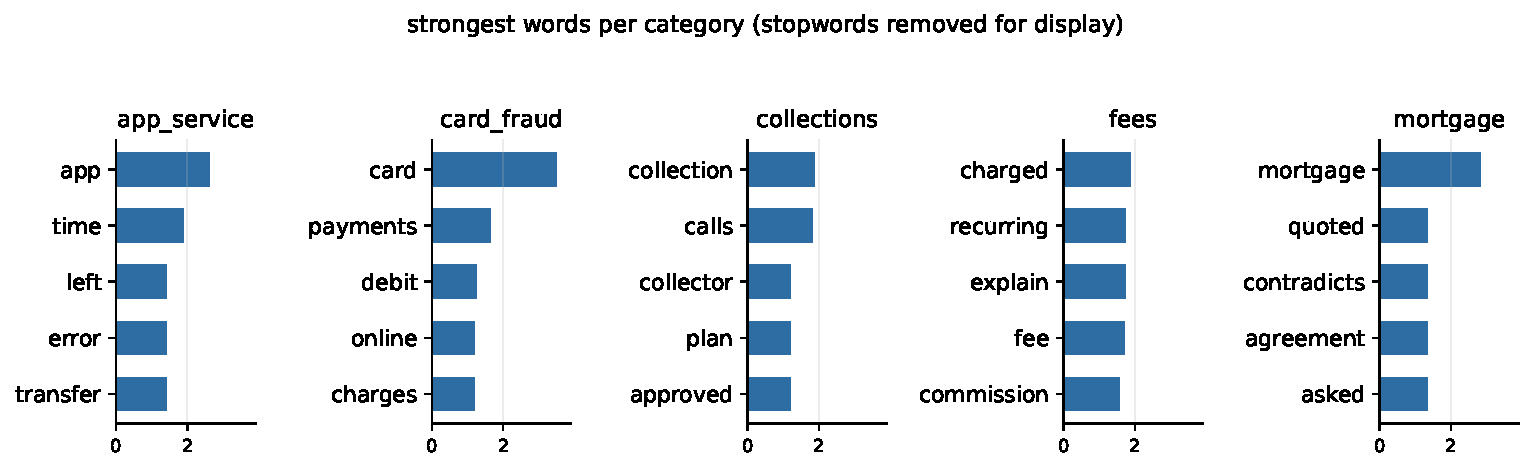
\includegraphics[width=0.98\textwidth]{figures/fig_class_words.pdf}
  \end{center}
  \begin{itemize}\small
    \item Top coefficients per class are a \alert{sanity check you can
          read}: fraud listens for \emph{card, payments, online};
          collections for \emph{collector, calls}; mortgage for
          \emph{agreement, contradicts}.
    \item An off-topic top word = the leakage smell, text edition
          (imagine \emph{refunded} predicting fraud - written
          \emph{after} resolution).
  \end{itemize}
\end{frame}

% ---------------------------------------------------------------
\begin{frame}{Multiclass metrics in one slide}
  \begin{itemize}
    \item \textbf{Per-class precision/recall} - five confusion-matrix
          rows; report the worst, not just the mean (the router's weakest
          queue is the one that pages you).
    \item \textbf{Macro-F1}: average F1 over classes, each class equal -
          the imbalance-honest default.
    \item \textbf{Weighted-F1 / accuracy}: dominated by big classes -
          fine only when classes are balanced (ours are, by
          construction).
    \item Thresholds exist here too: route automatically only above a
          confidence bar, send the rest to a \alert{human queue} - the
          expected-cost logic of Block 3, multiclass edition.
  \end{itemize}
\end{frame}

% ---------------------------------------------------------------
\begin{frame}{From accuracy to operations: the confidence bar}
  Route automatically only when the model is sure; queue the rest for
  humans. Our router, on the test set:
  \vspace{0.3em}
  \begin{center}\small
  \begin{tabular}{@{}cccc@{}}
    \toprule
    confidence bar & auto-routed & accuracy (auto) & human queue \\
    \midrule
    none & 100\% & 90.3\% & 0\% \\
    0.5 & 91\% & 93.6\% & 9\% \\
    \alert{0.6} & \alert{81\%} & \alert{98.3\%} & \alert{19\%} \\
    0.7 & 79\% & 100\% & 21\% \\
    \bottomrule
  \end{tabular}
  \end{center}
  \vspace{0.1em}
  \begin{itemize}\small
    \item The bar is Block 3's threshold logic, multiclass edition: trade
          automation volume against error cost, with the business.
    \item At a 0.6 bar: four in five complaints route themselves, nearly
          error-free - and the humans see only the genuinely hard fifth.
  \end{itemize}
\end{frame}

% ---------------------------------------------------------------
\begin{frame}{Naive Bayes: the classical text baseline (mention)}
  \begin{itemize}
    \item Counts word frequencies per class, multiplies probabilities as
          if words were independent - \alert{naively}; hence the name.
    \item Wrong assumption, strong baseline: fast, tiny, decent on small
          text data - for decades \emph{the} spam-filter algorithm.
    \item sklearn: \texttt{MultinomialNB}; one line to swap into our
          pipeline (notebook exercise - and the baseline discipline says
          you should).
  \end{itemize}
\end{frame}

% ---------------------------------------------------------------
\begin{frame}{Embeddings \& LLMs: the modern bridge (where it fits)}
  \begin{itemize}
    \item TF-IDF sees \emph{words}; embeddings see \emph{meaning} -
          ``the app crashes'' and ``application keeps freezing'' land close
          in embedding space, far in TF-IDF space.
    \item Modern practice: an embedding model (or LLM) turns text into
          dense vectors $\to$ the same classical models we already know.
          \alert{Block 2's ``LLMs as feature factories''}, delivered.
    \item TF-IDF still wins when: data is small, latency and cost matter,
          and the \alert{auditor asks why} - coefficients over vibes.
    \item Rule of the shop: start with TF-IDF + logistic; let embeddings
          \emph{earn} their complexity (the Block 3 discipline, verbatim).
  \end{itemize}
\end{frame}

% ============================================================
% SECTION: PITFALLS
% ============================================================
\section{Pitfalls}

% ---------------------------------------------------------------
\begin{frame}{The sobering demo, basket edition}
  We shuffled every product column independently - destroying all
  co-occurrence, keeping every penetration rate. Then mined with the same
  settings:
  \vspace{0.4em}
  \begin{center}
  \begin{tabular}{@{}lcc@{}}
    \toprule
     & real baskets & \alert{shuffled baskets} \\
    \midrule
    rules passing the same filters & 545 & \alert{312} \\
    best lift & 4.28 & \alert{1.14} \\
    \bottomrule
  \end{tabular}
  \end{center}
  \vspace{0.5em}
  \begin{itemize}\small
    \item The rule \emph{count} is nearly meaningless - the same filters
          pass \alert{three hundred ``rules''} on pure noise.
    \item What noise cannot fake is \alert{lift}: 1.14 versus 4.28. Rank by
          lift, and demand it clears noise levels - Block 4's noise
          question, answered with a number.
  \end{itemize}
\end{frame}

% ---------------------------------------------------------------
\begin{frame}{Text hygiene}
  \begin{itemize}
    \item \textbf{Vectoriser inside the pipeline} - vocabulary and idf
          are fitted parameters; fitting them on all data is leakage
          (rare-word idf especially).
    \item \textbf{Vocabulary drifts} - new products, new slang, new
          fraud patterns; a 2024 vocabulary reads 2026 complaints badly.
          Out-of-time testing applies to text too.
    \item \textbf{PII everywhere} - names, account numbers, phone
          numbers live inside free text; anonymise before mining, log
          nothing raw (GDPR is not a footnote).
    \item \textbf{Language reality} - our corpus is conveniently
          English; Polish morphology (\emph{opłata, opłaty, opłatom,
          opłatach}) makes lemmatisation earn its keep.
  \end{itemize}
\end{frame}

% ---------------------------------------------------------------
\begin{frame}{A word on Polish (and any inflected language)}
  \begin{itemize}
    \item Our corpus is conveniently English. Polish text multiplies every
          noun into a dozen surface forms - bag-of-words sees
          \emph{opłata} and \emph{opłatach} as strangers.
    \item Survival kit: lemmatisation with a Polish model (spaCy
          \texttt{pl\_core\_news}, Stanza, Morfeusz), diacritics kept
          (\emph{łata} $\ne$ \emph{lata}), and \alert{character n-grams}
          as the robust fallback - they shrug at inflection and typos.
    \item Embedding models are trained multilingually and largely dissolve
          the problem - one more genuine LLM-era win (previous slide's
          trade-offs still apply).
    \item Project note: mining Polish text is welcome - state your
          normalisation recipe explicitly.
  \end{itemize}
\end{frame}

% ---------------------------------------------------------------
\begin{frame}{Common sins of both crafts}
  \begin{enumerate}
    \item Reporting \textbf{confidence without lift} - base-rate
          flattery as insight.
    \item \textbf{One insight in ten costumes} - mirror and superset
          rules padding a slide deck.
    \item Reading rules \textbf{causally} - and designing an
          intervention that changes the pattern it relied on.
    \item \textbf{Stopword cargo-culting} - deleting words like
          \emph{not} (``not refunded''!) because a default list said so.
    \item \textbf{Evaluating text models on their own templates} -
          near-duplicate documents across the split; the duplicate leak,
          text edition.
    \item Shipping a router with \textbf{no human queue} - 90\% right
          means one complaint in ten lands on the wrong desk, silently.
  \end{enumerate}
\end{frame}

% ============================================================
% SECTION: LAB
% ============================================================
\section{Lab}

% ---------------------------------------------------------------
\begin{frame}[plain]
  \begin{center}
    \vspace{1.5cm}
    {\LARGE\textbf{Laboratory}}\\[0.6cm]
    {\normalsize Notebook \texttt{05\_pattern\_mining\_text} - laptops out.}
  \end{center}
\end{frame}

% ---------------------------------------------------------------
\begin{frame}{Lab today}
  \begin{columns}[T]
    \begin{column}{0.54\textwidth}
      \textbf{Notebook \texttt{05\_pattern\_mining\_text}}
      \begin{itemize}\small
        \item mine the product baskets: Apriori, rules, the
              lift-vs-confidence lesson
        \item run the shuffled-basket sobering check yourselves
        \item build the text bridge: counts $\to$ TF-IDF $\to$ n-grams
        \item train and audit the complaint router
      \end{itemize}
    \end{column}
    \begin{column}{0.44\textwidth}
      \textbf{Done =}
      \begin{itemize}\small
        \item three rules you would act on, with all three numbers and one
              honest sentence each
        \item a router whose confusion matrix you can \emph{explain}
      \end{itemize}
      \vspace{0.3em}
      \textbf{Optional extras}
      \begin{itemize}\small
        \item Naive Bayes bake-off
        \item cluster the complaints (Block 4 meets Block 5)
      \end{itemize}
    \end{column}
  \end{columns}
\end{frame}

% ============================================================
% SECTION: SUMMARY
% ============================================================
\section{Summary}

% ---------------------------------------------------------------
\begin{frame}[plain]
  \begin{center}
    \vspace{1.5cm}
    {\LARGE\textbf{Summary}}\\[0.6cm]
    {\normalsize What to take home from Block 5.}
  \end{center}
\end{frame}

% ---------------------------------------------------------------
\begin{frame}{Block 5 in five sentences}
  \begin{enumerate}
    \item Baskets are one abstraction - \textbf{transactions $\times$
          items} - and it fits far more than shopping.
    \item A rule has three numbers: \textbf{support} for materiality,
          \textbf{confidence} for the promise, \textbf{lift} for whether
          anything is there at all.
    \item \textbf{Apriori's} downward closure is why mining terminates
          before the universe does.
    \item Text becomes columns via \textbf{bag-of-words and TF-IDF} -
          and then the whole course applies, including the golden rule
          (vocabulary leaks too).
    \item Filters pass rules on noise and routers misfile one in ten -
          \textbf{honesty clauses ship with the deliverable}.
  \end{enumerate}
\end{frame}

% ---------------------------------------------------------------
\begin{frame}{Project status \& reminder - two weeks to go}
  \begin{itemize}
    \item Two weeks to the presentation - and remember the upload rule:
          \alert{all code + the final presentation, uploaded before Block 7
          starts}. Plan the polish time now, not on the last evening.
    \item This week's target: interpretation and a written recommendation;
          start the presentation skeleton. The presentation \& defence is
          \alert{20\% of the project grade} - budget real time for it.
    \item Text or baskets in your project? The honesty kit extends:
          lift over confidence, deduplicated rules, vectoriser in the
          pipeline, and one out-of-vocabulary sentence in the limitations.
    \item The rubric rewards \emph{correct and interpreted} over
          \emph{complex and mute} - today gave you two more interpretable
          tools, use them that way.
  \end{itemize}
\end{frame}

% ---------------------------------------------------------------
\begin{frame}{Exam practice - multiple choice}
  \small
  \textbf{Q1.} The rule savings $\Rightarrow$ checking has confidence 92.7\%
  and lift 1.00. Checking's overall penetration is 92.4\%. Act on the rule?
  \begin{enumerate}[(a)]
    \item yes - 92.7\% confidence is outstanding
    \item no - lift $\approx 1$ means savings tells us nothing beyond the
          base rate
    \item yes, but only for new customers
    \item cannot decide without support
  \end{enumerate}
  \vspace{0.4em}
  \textbf{Q2.} In TF-IDF, the idf factor:
  \begin{enumerate}[(a)]
    \item removes stop words from the vocabulary
    \item counts each word's frequency inside one document
    \item down-weights words appearing in many documents, up-weights
          distinctive ones
    \item normalises document length
  \end{enumerate}
\end{frame}
% Answer key: Q1 (b) - the confidence trap: high confidence purely inherited
% from a ubiquitous consequent; lift is the number that asks "beyond chance?".
% Q2 (c) - tf is the within-document count; idf is the cross-corpus rarity
% weight.

% ---------------------------------------------------------------
\begin{frame}{Exam practice - open question}
  \begin{block}{In the style of the term-0 exam ($\sim$60\% open questions)}
    Your complaint router ships at 90\% accuracy. Six months later the bank
    launches a new product, and complaints about it start arriving. Describe
    what happens to the router - loudly or silently? - and design the
    minimal monitoring that would catch it.
  \end{block}
  \vspace{0.5em}
  \begin{center}\small
    4-6 sentences. ``Retrain sometimes'' is not yet a design.
  \end{center}
\end{frame}
% A good answer: the failure is SILENT - the router has no "none of the
% above" class, so new-product complaints are confidently misfiled into the
% nearest old vocabulary; aggregate accuracy on old categories can even hold.
% Monitoring: track the prediction-confidence distribution (a growing
% low-confidence mass = novel text), per-class routing rates vs baseline,
% and a small ongoing human-labelled sample; retrain when confidence drifts
% or the sample's accuracy drops, not on a calendar.

% ---------------------------------------------------------------
\begin{frame}[plain]
  \begin{center}
    \vspace{1.5cm}
    {\LARGE\textbf{Next week: neural networks \& responsible ML.}}\\[0.6cm]
    {\normalsize The last new model family - and the questions that
    outlast every model.}
  \end{center}
\end{frame}

% ---------------------------------------------------------------
\begin{frame}{Keep learning - Block 5 reading}
  \begin{itemize}
    \item \textbf{Agrawal \& Srikant} - \emph{Fast Algorithms for Mining
          Association Rules} (VLDB 1994) - the original Apriori paper,
          still readable.
    \item \textbf{Sebastiani} - \emph{Machine Learning in Automated Text
          Categorization} (ACM Computing Surveys, 2002) - the classic
          survey behind today's router.
    \item \textbf{scikit-learn User Guide} - \emph{Working with text data}
          tutorial: our router pipeline, step by step.
    \item \textbf{mlxtend documentation} - the \texttt{frequent\_patterns}
          module: everything Apriori beyond today's lab.
  \end{itemize}
\end{frame}

\end{document}
